\chapter{anubaMdhagaLu}

\section*{\bfseries $2$ riMda $5000$ tanaka iruva aviBAjayx saMKeyxgaLu\\{\rm\bfseries Primes Numbers between 2 to 5000}}
\addcontentsline{toc}{section}{{\protect\bf anubaMdha $2$ riMda $5000$ tanaka iruva aviBAjayx saMKeyxgaLu}}

\begin{longtable}{>{$}l<{$}>{$}l<{$}>{$}l<{$}>{$}l<{$}>{$}l<{$}>{$}l<{$}>{$}l<{$}>{$}l<{$}>{$}l<{$}>{$}l<{$}}
%\multicolumn{9}{c}{\text{}}\\[0.3cm]
2    & 3    & 5    & 7    & 11   & 13   & 17   & 19   & 23\\
29   & 31   & 37   & 41   & 43   & 47   & 53   & 59   &61\\
67   & 71   & 73   & 79   & 83   & 89   & 97   & 101  & 103 \\
107  & 109  & 113  & 127  & 131  & 137  & 139  & 149  & 151\\
157  & 163  & 167  & 173  & 179  & 181  & 191  & 193  &197 \\    
199  & 211  & 223  & 227  & 229  & 233  & 239  & 241  &251 \\
257  & 263  & 269  & 271  & 277  & 281  & 283  & 293  &307 \\
311  & 313  & 317  & 331  & 337  & 347  & 349  & 353  &359 \\
367  & 373  & 379  & 383  & 389  & 397  & 401  & 409  &419 \\
421  & 431  & 433  & 439  & 443  & 449  & 457  & 461  &463 \\
467  & 479  & 487  & 491  & 499  & 503  & 509  & 521  &523 \\
541  & 547  & 557  & 563  & 569  & 571  & 577  & 587  &593 \\
599  & 601  & 607  & 613  & 617  & 619  & 631  & 641  &643 \\
647  & 653  & 659  & 661  & 673  & 677  & 683  & 691  &701 \\
709  & 719  & 727  & 733  & 739  & 743  & 751  & 757  &761 \\
769  & 773  & 787  & 797  & 809  & 811  & 821  & 823  &827 \\
829  & 839  & 853  & 857  & 859  & 863  & 877  & 881  &883 \\
887  & 907  & 911  & 919  & 929  & 937  & 941  & 947  &953 \\
967  & 971  & 977  & 983  & 991  & 997  & 1009 & 1013 &1019 \\
1021 & 1031 & 1033 & 1039 & 1049 & 1051 & 1061 & 1063 &    \\
1069 & 1087 & 1091 & 1093 & 1097 & 1103 & 1109 & 1117 &   \\
1123 & 1129 & 1151 & 1153 & 1163 & 1171 & 1181 & 1187 &   \\
1193 & 1201 & 1213 & 1217 & 1223 & 1229 & 1231 & 1237 &  \\
1249 & 1259 & 1277 & 1279 & 1283 & 1289 & 1291 & 1297 &  \\
1301 & 1303 & 1307 & 1319 & 1321 & 1327 & 1361 & 1367 &  \\
1373 & 1381 & 1399 & 1409 & 1423 & 1427 & 1429 & 1433 &  \\
1439 & 1447 & 1451 & 1453 & 1459 & 1471 & 1481 & 1483 &  \\
1487 & 1489 & 1493 & 1499 & 1511 & 1523 & 1531 & 1543 &  \\
1549 & 1553 & 1559 & 1567 & 1571 & 1579 & 1583 & 1597 &  \\
1601 & 1607 & 1609 & 1613 & 1619 & 1621 & 1627 & 1637 &  \\
1657 & 1663 & 1667 & 1669 & 1693 & 1697 & 1699 & 1709 &  \\
1721 & 1723 & 1733 & 1741 & 1747 & 1753 & 1759 & 1777 &  \\
1783 & 1787 & 1789 & 1801 & 1811 & 1823 & 1831 & 1847 &  \\
1861 & 1867 & 1871 & 1873 & 1877 & 1879 & 1889 & 1901 &  \\
1907 & 1913 & 1931 & 1933 & 1949 & 1951 & 1973 & 1979 &   \\
1987 & 1993 & 1997 & 1999 & 2003 & 2011 & 2017 & 2027 &  \\
2029 & 2039 & 2053 & 2063 & 2069 & 2081 & 2083 & 2087 &  \\
2089 & 2099 & 2111 & 2113 & 2129 & 2131 & 2137 & 2141 &  \\
2143 & 2153 & 2161 & 2179 & 2203 & 2207 & 2213 & 2224 &  \\
2237 & 2239 & 2243 & 2251 & 2267 & 2269 & 2273 & 2281 &  \\
2287 & 2293 & 2297 & 2309 & 2311 & 2333 & 2339 & 2341 &  \\
2347 & 2351 & 2357 & 2371 & 2377 & 2381 & 2383 & 2389 &  \\
2393 & 2399 & 2411 & 2417 & 2423 & 2437 & 2441 & 2447 &  \\
2459 & 2467 & 2473 & 2477 & 2503 & 2521 & 2531 & 2539 &  \\
2543 & 2549 & 2551 & 2557 & 2579 & 2591 & 2593 & 2609 &  \\
2617 & 2621 & 2633 & 2647 & 2657 & 2659 & 2663 & 2671 &  \\
2677 & 2683 & 2687 & 2689 & 2693 & 2699 & 2707 & 2711 &  \\
2713 & 2719 & 2729 & 2731 & 2741 & 2749 & 2753 & 2767 &  \\
2777 & 2789 & 2791 & 2797 & 2801 & 2803 & 2819 & 2833 &  \\
2837 & 2843 & 2851 & 2857 & 2861 & 2879 & 2887 & 2897 &  \\
2903 & 2909 & 2917 & 2927 & 2939 & 2953 & 2957 & 2963 &  \\
2969 & 2971 & 2999 & 3001 & 3011 & 3019 & 3023 & 3037 &  \\
3041 & 3049 & 3061 & 3067 & 3079 & 3083 & 3089 & 3109 &  \\
3119 & 3121 & 3137 & 3163 & 3167 & 3169 & 3181 & 3187 &  \\
3191 & 3203 & 3209 & 3217 & 3221 & 3229 & 3251 & 3253 &  \\
3257 & 3259 & 3271 & 3299 & 3301 & 3307 & 3313 & 3319 &  \\
3323 & 3329 & 3331 & 3343 & 3347 & 3359 & 3361 & 3371 &  \\
3373 & 3389 & 3391 & 3407 & 3413 & 3433 & 3449 & 3457 &  \\
3461 & 3463 & 3467 & 3469 & 3491 & 3499 & 3511 & 3517 &  \\
3527 & 3529 & 3533 & 3539 & 3541 & 3547 & 3557 & 3559 &  \\
3571 & 3581 & 3583 & 3593 & 3607 & 3613 & 3617 & 3623 &  \\
3631 & 3637 & 3643 & 3659 & 3671 & 3673 & 3677 & 3691 &  \\
3697 & 3701 & 3709 & 3719 & 3727 & 3733 & 3739 & 3761 &  \\
3767 & 3769 & 3779 & 3793 & 3797 & 3803 & 3821 & 3823 &  \\
3833 & 3847 & 3851 & 3853 & 3863 & 3877 & 3881 & 3889 &  \\
3907 & 3911 & 3917 & 3919 & 3923 & 3929 & 3931 & 3943 &  \\
3947 & 3967 & 3989 & 4001 & 4003 & 4007 & 4013 & 4019 &  \\
4021 & 4027 & 4049 & 4051 & 4057 & 4073 & 4079 & 4091 &  \\
4093 & 4099 & 4111 & 4127 & 4129 & 4133 & 4139 & 4153 &  \\
4157 & 4159 & 4177 & 4201 & 4211 & 4217 & 4219 & 4229 &  \\
4231 & 4241 & 4243 & 4253 & 4259 & 4261 & 4271 & 4273 &  \\
4283 & 4289 & 4297 & 4327 & 4337 & 4339 & 4349 & 4357 &  \\
4363 & 4373 & 4391 & 4397 & 4409 & 4421 & 4423 & 4441 &  \\
4447 & 4451 & 4457 & 4463 & 4481 & 4483 & 4493 & 4507 &  \\
4513 & 4517 & 4519 & 4523 & 4547 & 4549 & 4561 & 4567 &  \\
4583 & 4591 & 4597 & 4603 & 4621 & 4637 & 4639 & 4643 &  \\
4649 & 4651 & 4657 & 4663 & 4673 & 4679 & 4691 & 4703 &  \\
4721 & 4723 & 4729 & 4733 & 4751 & 4759 & 4783 & 4787 &  \\
4789 & 4793 & 4799 & 4801 & 4813 & 4817 & 4831 & 4861 &  \\
4871 & 4877 & 4889 & 4903 & 4909 & 4919 & 4931 & 4933 &  \\
4937 & 4943 & 4951 & 4957 & 4967 & 4969 & 4973 & 4987 &  \\
4993 & 4999 & \ldots &\ldots &\ldots &\ldots &\ldots &\ldots &  
\end{longtable}

\eject

\centerline{\text{veVdagaNitada sUtarxgaLu}}

\medskip

\begin{enumerate}[{\rm 1.}]
\item EkAdhikeVna pUveVRNa
\item niKilaM navatashacxramaM dashataH
\item UdhavxR tiyaRgABxyXmf
\item parAvatayxR yoVjayeVtf
\item shUnayxM sAmayx samucacxyeV
\item (AnurUpeyxV) shUnayxmanayxtf
\item saMkalana vayxvakalanABAyxmf
\item pUraNApUraNABAyxmf
\item calanakalanABAyxmf
\item yAvadUnamf
\item sheVSANayxMkeVna carameVNa
\item soVpAMtayxdavxyamaMtayxmf
\item EkanUyxneVna pUveVRNa
\item guNitasamucacxyaH
\item guNakasamucacxyaH
\end{enumerate}

\newpage

\section*{saMKeyxgaLa vagiVRkaraNa \\{\rm\bfseries Classification of Numbers}}
\addcontentsline{toc}{section}{{\protect\bf saMKeyxgaLa vagiVRkaraNa}}
\begin{figure}[H]
\centering
\includegraphics[scale=.82]{src/figure/165.eps}
\end{figure}

\newpage


\section*{vividha mAnagaLalilx saMKeyxgaLu\\{\rm\bfseries Numbers in Different Base Systems}}

\addcontentsline{toc}{section}{{\protect\bf vividha mAnagaLalilx saMKeyxgaLu }}
\textbf{dashamAnada oMdu saMKeyxge samanAda, divxmAna, paMcamAna, sapatxmAnada dAvxdashamAnada saMKeyxgaLu}

{\fontsize{9}{10}\selectfont
\tabcolsep=5pt
\renewcommand{\arraystretch}{.9}
\begin{longtable}[H]{|>{$}c<{$}|>{$}c<{$}|>{$}c<{$}|>{$}c<{$}|>{$}c<{$}|}
\multicolumn{1}{c}{$0 \cdots 9$} & \multicolumn{1}{p{2.7cm}}{\centering $0,1$} & \multicolumn{1}{c}{$0,1,2,3,4$} & \multicolumn{1}{c}{$0,1,2,3,4,5,6$}\\
\hline
\text{dashamAna} & \text{divxmAna} & \text{paMcamAna} & \text{sapatxmAna} & \text{dAvxdashamAna}\\
\hline
1   &   1     &   1 &  1   &   1 \\
\hline 
2   & (10)_2      &    2     &  2   &   2 \\
\hline
3   & (11)_2      &   3     &  3   &   3 \\
\hline
4   & (100)_2     &   4     &  4   &   4 \\
\hline
5   &  (101)_2    & (10)_5  &  5   &    5\\
\hline
6   &   (110)_2   & (11)_5  &  6   &    6\\
\hline
7   &   (111)_2   & (12)_5  &  (10)_7 & 7\\
\hline
8   &   (1000)_2  & (13)_5  & (11)_7  & 8\\
\hline
9   &   (1001)_2  & (14)_5  & (12)_7  & 9\\
\hline
10  &  (1010)_2   &  (20)_5  & (13)_7 & T \\
\hline
11  &  (1011)_2   &  (21)_5  &  (14)_7 & E\\
\hline
12  &  (1100)_2   &  (22)_5  &  (15)_7 & (10)_{12}\\
\hline
13  &  (1101)_2   &  (23)_5  &  (16)_7 & (11)_{12}\\
\hline
14  &  (1110)_2   &  (24)_5  &  (20)_7 & (12)_{12}\\
\hline
15  &  (1111)_2   &  (30)_5  &  (21)_7 &  (13)_{12}\\
\hline
16  &  (10000)_2  &   (31)_5 &  (22)_7 &  (14)_{12}\\
\hline
17  &  (10001)_2  &  (32)_5  &  (23)_7 & (15)_{12}\\
\hline
18  &  (10010)_2  &  (33)_5  &  (24)_7 &  (16)_{12}\\
\hline
19  &  (10011)_2  & (34)_5 &  (25)_7 &  (17)_{12}\\
\hline
20  &  (10100)_2  & (40)_5 & (26)_7  & (18)_{12}\\
\hline
21  &  (10101)_2  &  (41)_5 & (30)_7 & (19)_{12}\\
\hline
22  &  (10110)_2  &  (42)_5 & (31)_7 & (1T)_{12}\\
\hline
23  &  (10111)_2  &  (43)_5 & (32)_7 & (1E)_{12}\\
\hline
24  &  (11000)_2  &   (44)_5 & (33)_7 & (20)_{12}\\
\hline
25  &  (11001)_2  &   (100)_5 & (34)_7 & (21)_{12}\\
\hline
& \multicolumn{1}{p{2.7cm}|}{kAyxlfkuyxleVTarfnalilx upayoVgisuvudu  I padadhxtiyeV} & & &\\
\hline
\end{longtable}
}

\newpage

\section*{\hspace{3.5cm}pAriBASika padagaLu}

\addcontentsline{toc}{section}{{\protect\bf pAriBASika padagaLu }}

\begin{longtable}{>{\rm}l@{\hspace{1.25cm}}l}
Absolute & nirapeVkaSx\\
Abstract Number & amUtaRsaMKeyx\\
Addition & saMkalana\\
Aggregate & samaSiTx\\
Alternate & parAyxya\\
Analogy & anurUpate, sAdaqshayx\\
Analyse & vishelxVSisu\\
Appendix & anubaMdha\\
Application & anavxya \\
Approximate Value & saninxhita bele\\
Arithmetician & aMkagaNitajacnx\\
Ascending & Eruva, AroVhi\\
Average & sarAsari \\
Base Number & AdhAra saMKeyx\\
Basic Concept & mUlaparikalapxne\\
Basis & mUlAdhAra \\
Binomial Theorem & divxpadaparxmeVya\\
Bracket & AvaraNa\\
Calculus & kalanashAsatxrX\\
Calculation & lekAkxcAra, gaNane\\
Cardinal Number & gaNana saMKeyx\\
Classification & vagiVRkaraNa\\
Code & saMkeVta\\
Common Factor & sAmAnayx apavataRna\\
Comparision & tulane, hoVlike\\
Complex Number & saMkiVNaRsaMKeyx\\
Composite Number & BAjayx saMKeyx\\
Consecutive Numbers & anukarxma saMKeyxgaLu,\\
                    & karxmAgata saMKeyxgaLu\\
Constant Number & sithxrasaMKeyx\\
Count & eNisu\\
Counting Numbers & eNike saMKeyxgaLu\\
Cube & Gana\\
Cube Root & GanamUla\\
Cube Numbers & GanasaMKeyxgaLu\\
Cyclic & cakirxVya\\
Cyclic Numbers & cakirxVya saMKeyxgaLu\\
Decimal Numbers & dashamAMsha saMKeyxgaLu\\
Definition & vAyxKeyx\\
Denominator & CeVda\\
Descending & avaroVhaNa\\
Digit & aMka\\
Divisibility & BAjayxte\\
Divisor & BAjaka\\
Equality & samate, samAnate\\
Equal Numbers & samAna saMKeyxgaLu\\
Equation & samiVkaraNa\\
Equilateral Triangle & samabAhu tirxBuja\\
Error & tapupx, doVSa\\
Estimate & aMdAju\\
Even Number & samasaMKeyx\\
Factor & apavataRna\\
Formula & sUtarx\\
Furmat Last Theorem & PamaRna kaDeya parxmeVya\\
Fibonacci Numbers & PiboVnAkikx saMKeyxgaLu\\
Formula & sUtarx, saMkeSxVpoVkitx\\
Fundamental Operation & mUlaparikamaR\\
Generalisation & sAvaRtirxVkaraNa\\
Highest Common Factor & mahatatxma sAmAnayx apavataRna\\
Hindu Arabic Numerals & hiMdU arabibxV saMKAyx sUcakagaLu\\
Identical & savaRsamatavxda, ananayx\\
Identity Equation & nitayxsamiVkaraNa\\
Imaginary Number & UhAsaMKeyx; kAlapxnika saMKeyx\\
Indefinite & anidiRSaTx\\
Imaginary Numbers & kAlapxnika saMKeyx\\
Index & GAtasUci; sUci\\
Indivisible & aviBAjayx\\
Inequality & asamAnate\\
Inference & tiVmARna\\
Irrational Number & aBAgalabadhx saMKeyx\\
Integer & pUNARMka\\
Inverse & viloVma\\
Kaprekar Number & kaperxVkarf saMKeyx\\
Lowest Common Multiple & laGutama sAmAnayx apavatayxR\\
Magic Square & mAyAcwka\\
Mathematician & gaNitajacnx\\
Mathematics & gaNita\\
Minimum & kaniSaThx\\
Mixed Fraction & misharxBinanxrAshi\\
Multiple & apavatayxR\\
Multiplier & guNaka\\
Multiply & guNisu\\
Natural Numbers & sAvxBAvika saMKeyxgaLu\\
Negative Numbers & QuNasaMKeyxgaLu\\
Negative Sign & QuNacihenx\\
Negative Integer & QuNa pUNARMka\\
Negative Term & QuNapada\\
Number & saMKeyx\\
Numberline & saMKAyxreVKe\\
Numeral & saMKAyx sUcaka\\
Odd Number & besasaMKeyx\\
Operation & saMkirxye\\
Ordinal Number & karxmasUcaka saMKeyx\\
Palindrome & mAlA saMKeyx\\
Perfect Number & paripUNaRsaMKeyx\\
Positive Integer & dhanapUNARMka\\
Positive Number & dhanAMsha, dhanasaMKeyx\\
Prime Number & aviBAjayx saMKeyx\\
Pythagorian Numbers  & peYthAgoriyanf saMKeyxgaLu\\
Quotient & BAgalabadhx\\
Ramanujan Numbers & rAmAnujanf saMKeyxgaLu\\
Rational Number & BAgalabadhx saMKeyx\\
Real Number & neYjasaMKeyx, vAsatxva saMKeyx;\\
Rectangle & Ayata\\
Recurring Decimal & AvataRka dashamAMsha\\
Remainder & sheVSa\\
Remainder Theorem & sheVSa parxmeVya\\
Result & PalitAMsha\\
Right Angle & laMbakoVna\\
Root & mUla\\
Rule & niyama\\
Sign & cihenx\\
Simple Equation & saraLa samiVkaraNa\\
Simplification & saraLiVkaraNa\\
Simplify & saMkeSxVpisu\\
Square & vagaR\\
Square root & vagaRmUla\\
Theory of Numbers & saMKAyxshAsatxrX; saMKAyx sidAdhxMta\\
Triangular Numbers & tirxBujAkAra saMKeyxgaLu\\
Transpose & sathxLAMtarisu\\
Unequal & asama\\
Unique & EkeYka, ananayx\\
Unknown Number & ajAcnxta saMKeyx; avayxkatxsaMKeyx\\
Variable Number & carasaMKeyx\\
Whole Number & pUNaRsaMKeyx\\
Zero & sonenx
\end{longtable}

\eject
\section*{\hspace{4.5cm}garxMthaQuNa}

\addcontentsline{toc}{section}{{\protect\bf garxMthaQuNa }}
`saMKAyx parxpaMca' pusatxkakAkxgi I muMde namUdisiruva garxMthagaLa sahAyavanunx paDedidedxVne. pusatxkada leVKakarigU, parxkAshakarigU nananx kaqtajacnxtegaLu.

\medskip
\begin{tabular}{>{\rm }ll@{\hspace{0.9cm}}l}
1) & saMKAyxloVka      & shirxV enf. subarxmaNayx\\[0.2cm]
2) & saMKoyxVdhAyxna    & shirxV bi. siVtArAmashAsitxrX\\[0.2cm]
3) & saMKAyxvinoVda    & porx|| vi. ke. doresAvxmi \\[0.2cm]
4) & gaNitashAsatxrXda savxrUpa &  DA| si. enf. shirxVnivAsa ayayxMgArf\\[0.2cm]
5) & mAyAcwkagaLa  & DA| esf. bAlacaMdarxrAvf,\\   
   &  sAvxrasayx   & \qquad emf. sheYlaja,\\
   &               & \qquad vi. vanajA\\[0.2cm]
6) & aMki-saMKeyxgaLa  & bi. ke. vishavxnAtharAvf \\ 
   & sAmArxjayxdalilx  & ka. rA. vi. pa. beMgaLUru\\[0.2cm]
7) & saMKAyxvinAyxsa matutx & veY. esf. subarxhamxNayx\\
   & aviBAjayx saMKeyxgaLu   &                          \\[0.2cm]
8) & mAyAcwkagaLa sAvxrasayx & bi. ke. vishavxnAtharAvf\\
   &                         & ka. rA. vi. pa. beMgaLUru\\[0.2cm]
9) & catuvaNaRsamaseyx       & porx|| ji. Ti. nArAyaNarAvf\\[0.2cm]
10)&gaNitashAsatxrXcariterx  & DA| si. enf. shirxVnivAsa ayayxMgArf\\
   &                         & meYsUru vishavxvidAyxnilaya      
\end{tabular}


\vfill
\section*{ideV leVKakara parxkaTita kaqtigaLu}

\addcontentsline{toc}{section}{{\protect\bf ideV leVKakara parxkaTita kaqtigaLu}}
\begin{enumerate}[{\rm 1)}]
\item vijAcnxna keYpiDi (janapirxya vijAcnxna)
\item vijAcnxna oMdu pakiSxnoVTa
\item vijAcnxna veYvidhayx
\item vijAcnxna keYpiDi (pwrxDhashAlA vidAyxthiRgaLige)
\item AroVgayx-parisara-paradhamaR
\item gaNita mAdhuyaR
\item meduLige kasaratutx (gaNitada samaseyxgaLu)
\item gaNita agaNita
\item saMKAyxvinAyxsa matutx aviBAjayx saMKeyxgaLu
\item nAveSuTx budidhxvaMtaru (gaNitakekx saMbaMdhisidaMte)
\item makakxLa keYcaLaka (reVKAgaNitakekx saMbaMdhisidaMte)
\item jagatitxna parxKAyxta gaNitajacnxru.
\item gaNita veYvidhayx 
\item gaNitada nUtana mAdari parxshenxgaLu
\end{enumerate}
